\documentclass{article}
\usepackage[margin=1in]{geometry}
\usepackage{amsmath,amsthm,amssymb}
\usepackage{bbm,enumerate,mathtools}
\usepackage{tikz,pgfplots}
\usepackage{chessboard}
\usepackage[hidelinks]{hyperref}
\usepackage{multicol} % Problem 35
\usepackage{xstring} % Difficulty command
\usetikzlibrary{shapes.geometric}

\newenvironment{question}{\begin{trivlist}\item[\textbf{Question.}]}{\end{trivlist}}
\newenvironment{note}{\begin{trivlist}\item[\textbf{Note.}]}{\end{trivlist}}
\newenvironment{references}{\begin{trivlist}\item[\textbf{References.}]}{\end{trivlist}}
\newenvironment{related}{\begin{trivlist}\item[\textbf{Related.}]\end{trivlist}\begin{enumerate}}{\end{enumerate}}

\newcommand\score[1]{
\pgfmathsetmacro\pgfxa{#1+1}
\tikzstyle{scorestars}=[
  star,
  star points=5,
  star point ratio=2.25,
  draw,
  inner sep=3pt,
  anchor=outer point 5
]
  \begin{tikzpicture}[baseline]
    \draw[opacity=0] (0,-0.5) rectangle (0,0.2); % Workaround for whitespace at the bottom.
    \foreach \i in {1,...,4} {
      \pgfmathparse{(\i<=#1?"yellow":"gray")}
      \edef\starcolor{\pgfmathresult}
      \draw (\i*4.5ex,0) node[name=star\i,scorestars,fill=\starcolor]  {};
    }
  \end{tikzpicture}
}

\newcommand{\difficulty}[1]{%
  \IfEqCase{#1}{%
      {1}{
        
\begin{tikzpicture}[scale=0.7, baseline=0.9mm]%
          \definecolor{slopegreen}{rgb}{0.0, 0.5, 0.0}%
          \fill[slopegreen] (0.5,0.5) circle (0.5);%
        \end{tikzpicture}%
      }%
      {2}{
        
\begin{tikzpicture}[scale=0.7, baseline=0.9mm]%
          \definecolor{slopeblue}{rgb}{0.0, 0.44, 1.00}
          \fill[slopeblue] (0,0) rectangle (1,1);%
        \end{tikzpicture}%
      }%
      {3}{
\begin{tikzpicture}[scale=0.7, baseline=0.9mm]\fill (0,0.5)--(0.5, 0)--(1,0.5)--(0.5,1)--cycle; \end{tikzpicture}}%
      {4}{
\begin{tikzpicture}[scale=0.7, baseline=0.9mm]\fill (0.25,0)--(0,0.5)--(0.25,1)--(0.5,0.5)--cycle; \fill (0.75,0)--(0.5,0.5)--(0.75,1)--(1,0.5)--cycle;\end{tikzpicture}}%
      % you can add more cases here as desired
  }[\PackageError{difficulty}{Undefined difficulty level: #1}{}]%
}%
\newcommand{\rating}[2]{\difficulty{#1}\\\score{#2}\\}


\begin{document}
\rating{3}{2}
Consider all of the shapes that can be made with a rubber band and a rubber
hand.

\begin{figure}[!h]
  \centering
  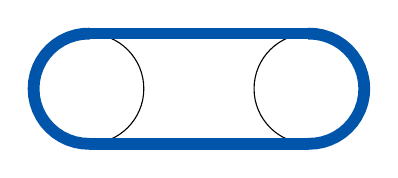
\begin{tikzpicture}[scale=0.7]
    \draw (0,0) circle (1);
    \draw (4,0) circle (1);
    \draw[line width=0.15cm, draw={rgb:green,1;blue,2}, domain=89:271] plot ({1*cos(\x) + 0}, {1*sin(\x) + 0});
    \draw[line width=0.15cm, draw={rgb:green,1;blue,2}] (0,1) -- (4,1);
    \draw[line width=0.15cm, draw={rgb:green,1;blue,2}, domain=-91:91] plot ({1*cos(\x) + 4}, {1*sin(\x) + 0});
    \draw[line width=0.15cm, draw={rgb:green,1;blue,2}] (0,-1) -- (4,-1);
  \end{tikzpicture}
  \hspace{0.5cm}
  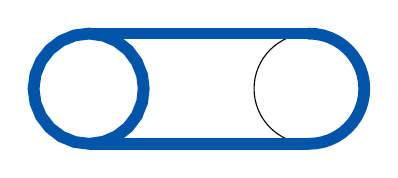
\begin{tikzpicture}[scale=0.7]
    \draw (0,0) circle (1);
    \draw (4,0) circle (1);
    \draw[line width=0.15cm, draw={rgb:green,1;blue,2}, domain=-1:361] plot ({1*cos(\x) + 0}, {1*sin(\x) + 0});
    \draw[line width=0.15cm, draw={rgb:green,1;blue,2}] (0,1) -- (4,1);
    \draw[line width=0.15cm, draw={rgb:green,1;blue,2}, domain=-91:91] plot ({1*cos(\x) + 4}, {1*sin(\x) + 0});
    \draw[line width=0.15cm, draw={rgb:green,1;blue,2}] (0,-1) -- (4,-1);
  \end{tikzpicture}
  \hspace{0.5cm}
  
\begin{tikzpicture}[scale=0.7]
    \draw (0,0) circle (1);
    \draw (4,0) circle (1);
    \draw[line width=0.15cm, draw={rgb:green,1;blue,2}, domain=-1:361] plot ({1*cos(\x) + 0}, {1*sin(\x) + 0});
    \draw[line width=0.15cm, draw={rgb:green,1;blue,2}] (0,1) -- (4,1);
    \draw[line width=0.15cm, draw={rgb:green,1;blue,2}, domain=-1:361] plot ({1*cos(\x) + 4}, {1*sin(\x) + 0});
    \draw[line width=0.15cm, draw={rgb:green,1;blue,2}] (0,-1) -- (4,-1);
  \end{tikzpicture}
  \\~\\
  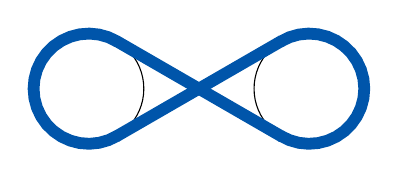
\begin{tikzpicture}[scale=0.7]
    \draw (0,0) circle (1);
    \draw (4,0) circle (1);
    \draw[line width=0.15cm, draw={rgb:green,1;blue,2}, domain=59:301] plot ({1*cos(\x) + 0}, {1*sin(\x) + 0});
    \draw[line width=0.15cm, draw={rgb:green,1;blue,2}, domain=-121:121] plot ({1*cos(\x) + 4}, {1*sin(\x) + 0});
    \draw[line width=0.15cm, draw={rgb:green,1;blue,2}, domain=-1.5:1.5] plot ({\x + 2}, {tan(30)*\x});
    \draw[line width=0.15cm, draw={rgb:green,1;blue,2}, domain=-1.5:1.5] plot ({\x + 2}, {-tan(30)*\x});
  \end{tikzpicture}
  \hspace{0.5cm}
  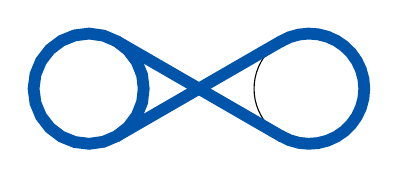
\begin{tikzpicture}[scale=0.7]
    \draw (0,0) circle (1);
    \draw (4,0) circle (1);
    \draw[line width=0.15cm, draw={rgb:green,1;blue,2}, domain=-1:361] plot ({1*cos(\x) + 0}, {1*sin(\x) + 0});
    \draw[line width=0.15cm, draw={rgb:green,1;blue,2}, domain=-121:121] plot ({1*cos(\x) + 4}, {1*sin(\x) + 0});
    \draw[line width=0.15cm, draw={rgb:green,1;blue,2}, domain=-1.5:1.5] plot ({\x + 2}, {tan(30)*\x});
    \draw[line width=0.15cm, draw={rgb:green,1;blue,2}, domain=-1.5:1.5] plot ({\x + 2}, {-tan(30)*\x});
  \end{tikzpicture}
  \hspace{0.5cm}
  
\begin{tikzpicture}[scale=0.7]
    \draw (0,0) circle (1);
    \draw (4,0) circle (1);
    \draw[line width=0.15cm, draw={rgb:green,1;blue,2}, domain=-1:361] plot ({1*cos(\x) + 0}, {1*sin(\x) + 0});
    \draw[line width=0.15cm, draw={rgb:green,1;blue,2}, domain=-1:361] plot ({1*cos(\x) + 4}, {1*sin(\x) + 0});
    \draw[line width=0.15cm, draw={rgb:green,1;blue,2}, domain=-1.5:1.5] plot ({\x + 2}, {tan(30)*\x});
    \draw[line width=0.15cm, draw={rgb:green,1;blue,2}, domain=-1.5:1.5] plot ({\x + 2}, {-tan(30)*\x});
  \end{tikzpicture}
  \\~\\
  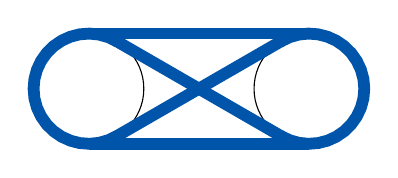
\begin{tikzpicture}[scale=0.7]
    \draw (0,0) circle (1);
    \draw (4,0) circle (1);
    \draw[line width=0.15cm, draw={rgb:green,1;blue,2}, domain=59:301] plot ({1*cos(\x) + 0}, {1*sin(\x) + 0});
    \draw[line width=0.15cm, draw={rgb:green,1;blue,2}] (0,1) -- (4,1);
    \draw[line width=0.15cm, draw={rgb:green,1;blue,2}, domain=-121:121] plot ({1*cos(\x) + 4}, {1*sin(\x) + 0});
    \draw[line width=0.15cm, draw={rgb:green,1;blue,2}] (0,-1) -- (4,-1);
    \draw[line width=0.15cm, draw={rgb:green,1;blue,2}, domain=-1.5:1.5] plot ({\x + 2}, {tan(30)*\x});
    \draw[line width=0.15cm, draw={rgb:green,1;blue,2}, domain=-1.5:1.5] plot ({\x + 2}, {-tan(30)*\x});
  \end{tikzpicture}
  \hspace{0.5cm}
  
\begin{tikzpicture}[scale=0.7]
    \draw (0,0) circle (1);
    \draw (4,0) circle (1);
    \draw[line width=0.15cm, draw={rgb:green,1;blue,2}, domain=-1:361] plot ({1*cos(\x) + 0}, {1*sin(\x) + 0});
    \draw[line width=0.15cm, draw={rgb:green,1;blue,2}] (0,1) -- (4,1);
    \draw[line width=0.15cm, draw={rgb:green,1;blue,2}, domain=-121:121] plot ({1*cos(\x) + 4}, {1*sin(\x) + 0});
    \draw[line width=0.15cm, draw={rgb:green,1;blue,2}] (0,-1) -- (4,-1);
    \draw[line width=0.15cm, draw={rgb:green,1;blue,2}, domain=-1.5:1.5] plot ({\x + 2}, {tan(30)*\x});
    \draw[line width=0.15cm, draw={rgb:green,1;blue,2}, domain=-1.5:1.5] plot ({\x + 2}, {-tan(30)*\x});
  \end{tikzpicture}
  \hspace{0.5cm}
  
\begin{tikzpicture}[scale=0.7]
    \draw (0,0) circle (1);
    \draw (4,0) circle (1);
    \draw[line width=0.15cm, draw={rgb:green,1;blue,2}, domain=-1:361] plot ({1*cos(\x) + 0}, {1*sin(\x) + 0});
    \draw[line width=0.15cm, draw={rgb:green,1;blue,2}] (0,1) -- (4,1);
    \draw[line width=0.15cm, draw={rgb:green,1;blue,2}, domain=-1:361] plot ({1*cos(\x) + 4}, {1*sin(\x) + 0});
    \draw[line width=0.15cm, draw={rgb:green,1;blue,2}] (0,-1) -- (4,-1);
    \draw[line width=0.15cm, draw={rgb:green,1;blue,2}, domain=-1.5:1.5] plot ({\x + 2}, {tan(30)*\x});
    \draw[line width=0.15cm, draw={rgb:green,1;blue,2}, domain=-1.5:1.5] plot ({\x + 2}, {-tan(30)*\x});
  \end{tikzpicture}
  \caption{
    There are (at least) 9 ways to weave a rubber band between two fingers up to
    reflection/rotation.
  }
\end{figure}

\begin{question}
  How many figures can be made with $n$ fingers and a rubber band?
\end{question}
\begin{related}
  \item Is there an analog in higher dimensions?
  \item What if all fingers must be aligned?
  \item What if all fingers must be on the corners of an $n$-gon?
\end{related}
\end{document}
